\documentclass[
        a4paper,
        10pt,
        parskip = full,    % Layout with zero \parident and non-zero \parskip
    ]{scrartcl}
% \usepackage[utf8]{inputenc}

\usepackage[top=2cm, bottom=2.5cm, left=2.5cm, right=2.5cm]{geometry}
\usepackage[
        colorlinks = true,    % Disable drawing boxes around links.
        linkcolor = black,    % Sets the color of links to black.
    ]{hyperref}
\usepackage{amsmath}
\usepackage{graphicx}
\usepackage{subfig}
\usepackage{float}

\begin{document}

\textbf{\large{Laboratory - Deep Learning Lab, WS 2018/2019 - Exercise 2}}

\textbf{\large{Submitted by: Amadeus Hovekamp,\\
amadeus.hovekamp@rwth-aachen.de,\\
Matr. no: 4603934}}

The repository with the source code can be found under the following link:\\
\href{https://github.com/Schokokugel/RoboticsLab}
     {https://github.com/Schokokugel/RoboticsLab}

\section{Running the default network and testing smaller batch sizes}
The default settings for training the network are 12 trainings epochs using the
complete training set with 50000 samples, a learning rate of $10^{-3}$ and
batches of size 128. The two 2d convolution layers both consist of 16 filters of
size $3 \times 3$. The validation set contains 10000 and the final test set
10000 samples.

When I ran this network on my CPU for the first time, I achieved a very good
performance even after only a single epoch, reaching more than 98 \% accuracy.
But when I managed to run the network on my GPU (NVIDIA GeForce GTX 950M, Ubuntu
18.04), the accuracy on the validation set reached barely 82 \% after one epoch
using the exact same code. Before I continued with task 2 I therefore checked,
if the batch size of 128 might be the reason of low performance, because the
resulting tensorflow graph might be too big to fit in the available 3.6 GB of
graphic memory.

\begin{figure}[H]
	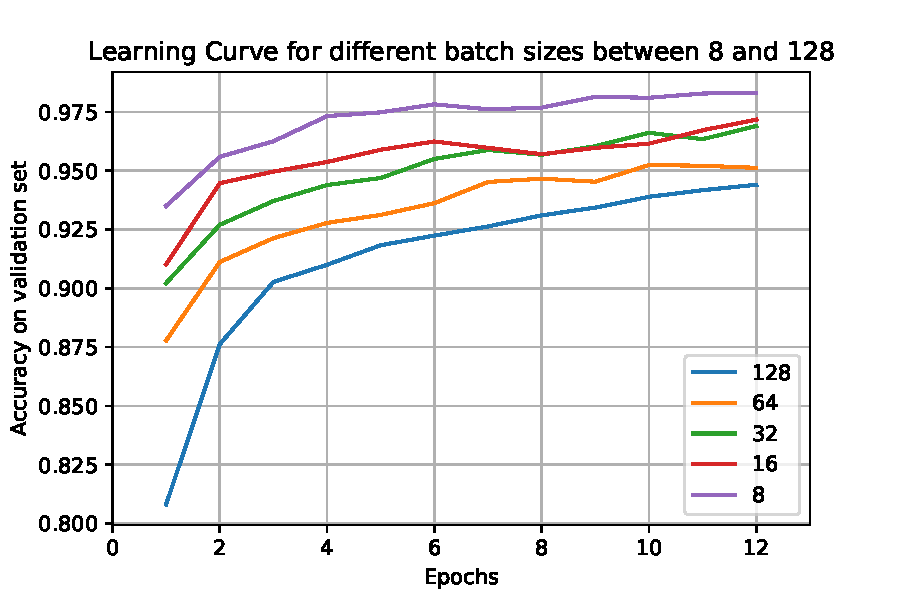
\includegraphics{../images/Learning_curve_for_Batch_Sizes.pdf}
	\caption{Learning curve for the default network}
  \label{BatchSize}
\end{figure}

Figure \ref{BatchSize} shows a connection between convergence speed and batch
size, but where this difference comes from, I do not know. Using smaller batch
sizes in the current implementation leads to more gradient steps in one epoch,
which might a reason for this performance difference.

\section{Learning rate experiments}
Even though the batch size had a big influence of the network's performance, I
used the default settings for the experiments and only changed the learning rate.
The results are shown in Figure \ref{LearningRate}.

\begin{figure}[H]
	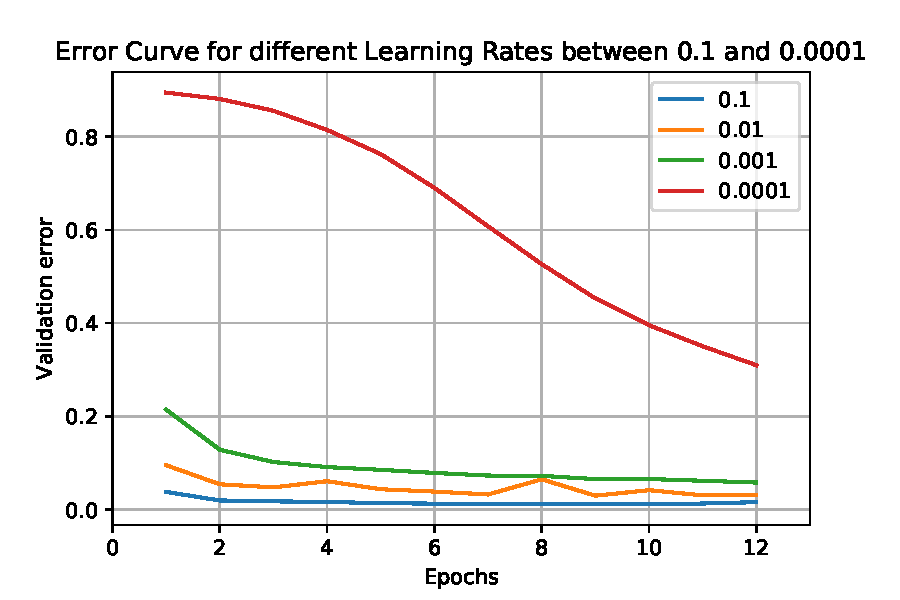
\includegraphics{../images/Error_curve_for_Learning_Rates.pdf}
	\caption{Error Curve for different Learning Rates between 0.1 and 0.0001}
  \label{LearningRate}
\end{figure}

One instantly sees the big difference between the smallest learning rate of
$10^{-4}$ and the bigger learning rates. A learning rate that small might slow
down the learning of a network very much. After one epoch the network barely
performes better than random (which would yield an error rate about 0.9). After
12 epochs it still performes much worse than the other three networks after a
single epoch of training. The other three networks perform similar but still one
can see a trend: A bigger learning rate yields better results. Generally this is
not true, because when the learning rate is set too big, the steps of the
gradient descent algorithm might jump over valleys of the loss function and thus
oscillate around a minimum or possibly even diverge if the step size is way too
big.

\section{Filter size experiments}
In this experiment I only changed the filter size of the convolution layers. All
filters in the two 2d convolution layers is of size $filtersize \times filtersize$.
Figure \ref{LearningRate} shows the results. The learning process of all networks
looks similar but from the second epoch onwards on sees that a higher filter size
leads to performance improvements.

\begin{figure}[H]
	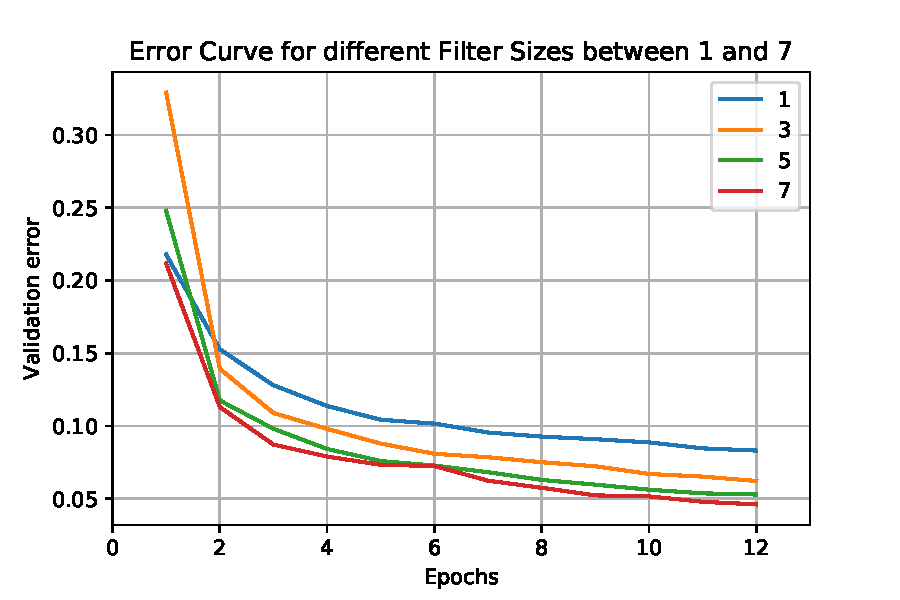
\includegraphics{../images/Error_curve_for_Filter_Sizes.pdf}
	\caption{Error Curve for different Filter Sizes between 1 and 7}
  \label{FilterSize}
\end{figure}
 The higher filter size enables the network to recognize features of bigger size.
 A network with bigger filters is generally more powerful but also has more
 parameters which requires more computation to train it. Therefore the size of
 the filters used should match the size of the features those filters have to
 detect: Small features $\rightarrow$ small filters. Large features $\rightarrow$
 large filters.

 Deep convolution networks might learn these bigger features by combining
 several smaller features from the layer before. This way the filters of size 3
 and 5 perform just a little worse than the filter of size 7.

\section{Random search}
In Figure \ref{RandomSearch} the results of 50 iterations of random search are
shown. The red line displays the performance of the best configuration trained
for 6 epochs found upto that iteration. Some somewhat good networks have been
found by the random search, the best iteration being iteration 18.

\begin{figure}
	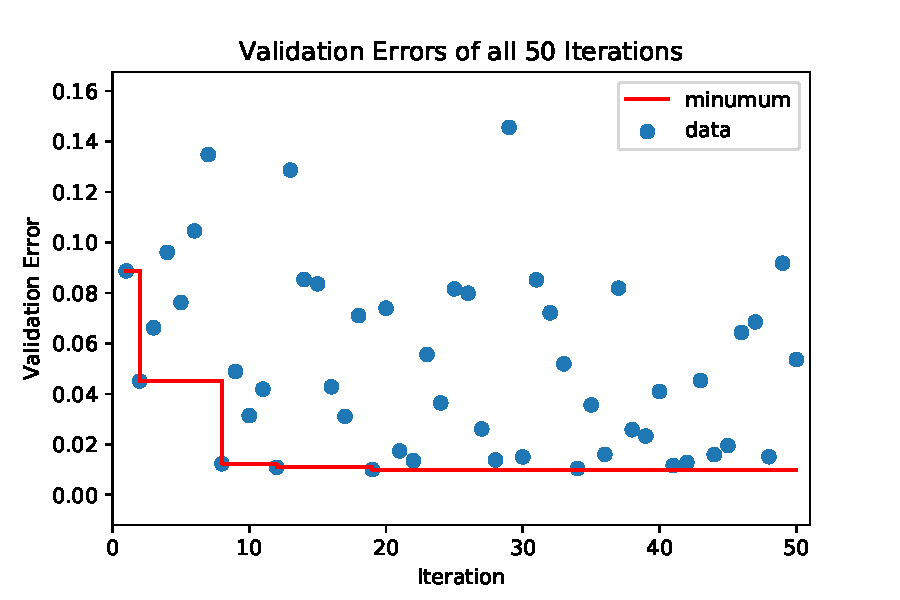
\includegraphics{../images/ah_random_search.pdf}
	\caption{Validation Error for all 50 Iterations of Random Search}
  \label{RandomSearch}
\end{figure}

When comparing the results of the best iterations of random search with the
networks tested in task 1 and task 2 one can see that only the default network
with a learning rate of 0.1 achieved similarly good performances on the
validation set. This shows that when there is little knowledge of how the
hyperparameters should be set for a specific problem, random search is a very
useful approach to find good hyperparameter settings. One big downside is the
long computation time which in my case was 220 minutes for 50 iterations and 6
epochs each, about 4.4 minutes per iteration. One can notice too, that the last
32 iterations, more than half of the total number of iterations did not improve
the best configuration found so far.

Figure \ref{RandomSearchBestConfig} shows the learning curve of a network
trained with the best set of parameters found in iteration 18 of the random
search. It has a rather small filter size but a relatively big learning rate
and medium sized batch size. The performence is nearly the same as in the random
search iteration, but one can see oszillations in the validation error, probably
due to the rather large learning rate. The error on the test set is
0.009599983 which is just as good as the performance on the validation set.

\begin{figure}
	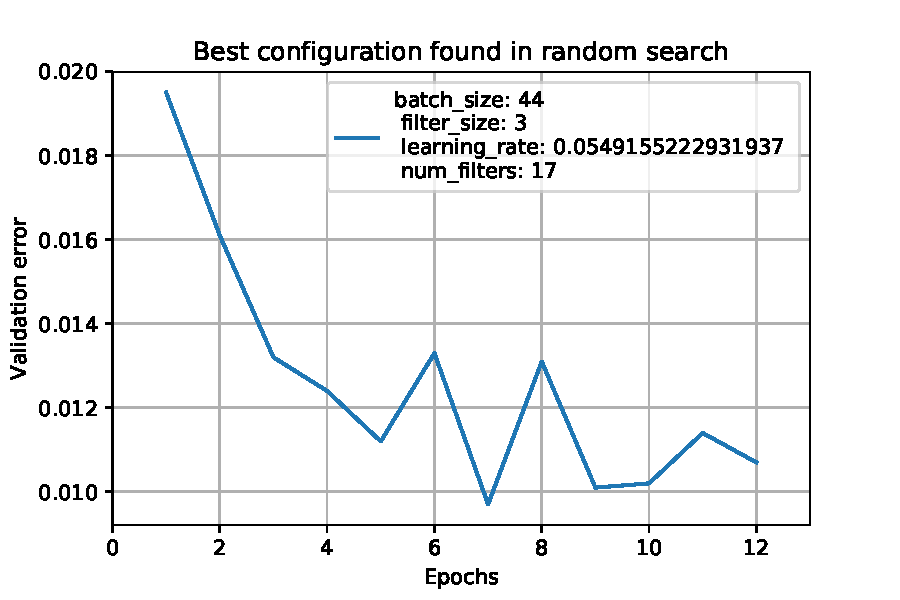
\includegraphics{../images/Random_Search_Best_Configuration.pdf}
	\caption{Validation Error of the best hyperparameter set found with Random Search}
  \label{RandomSearchBestConfig}
\end{figure}

\end{document}
